%============================================================================================================================
%............................................................................................................................
% Plantilla de Reportes - Ing. Edwin Rosario Gabriel
% UPIBI - Ingenieria Biomédica - Electronica I
%............................................................................................................................
%============================================================================================================================

\documentclass[12pt,spanish]{article}
\usepackage{etex}  % Para evitar problemas de too many package
\usepackage{floatrow}  % Para poner una tabla al lado de una figura
\usepackage{float}  % Para fijar las imagenes como flotantes
\usepackage{amsfonts,amsmath,amssymb,amsthm,latexsym,amstext,commath} % Paquetes de matematicas
\usepackage[spanish, es-tabla]{babel}  % Cambia de Idioma Chapter 1 a Capítulo 1 y div las palabras
\usepackage{parskip}  % Para quitar la sangria de cada parrafo sin poner \noindent
\usepackage[utf8]{inputenc}  % Para  acentos y las eñes cuando la codificacion en UTF-8
\usepackage{helvet}  % Cambio global de la Fuente
\usepackage{graphicx}  % Para los graficos e imagenes
\usepackage{verbatim}  % Para -comment- y tambien p/imp tal cual fue digitado
\usepackage{setspace}  % Para fijar el espaciado entre los parrafos.
\usepackage{fancyhdr}  % para los headers
\usepackage{color}  % Para los colores
\usepackage{listings}  % Para poner los codigos
\usepackage{subfigure}  % Para unir varias imagenes en una solo Fig
\usepackage{multicol}  % Para multicolumnass
\usepackage{epstopdf}  % Para convertir imagenes eps a pdf
\usepackage{wrapfig}  % Para poner figuras al lado del texto
\usepackage[rflt]{floatflt}  % Figuras flotantes entre el texto
\usepackage{mathtools}									
\usepackage[top=2.5cm,bottom=2.5cm,lmargin=3.5cm,rmargin=2.5cm]{geometry} % Especifica el diseño del documento.
\usepackage[export]{adjustbox}                               % Para center, left, right de las fig. en ambiente figure{}
\usepackage{tabularx}                                        % Para fijar ancho de las tablas cuando el texto es grande
\usepackage{booktabs}                                        % Para cambiar aspecto de las lineas horizon de las tablas
\usepackage{fixltx2e}					%Para subindices y superindices
\usepackage{gensymb}				%Para símbolos especiales
\renewcommand{\baselinestretch}{2}						 	 % Interlineado del documento
\newfloatcommand{capbtabbox}{table}[][\FBwidth]
%===========================================================================================================================
%............................................................................................................................
\begin{document}
	%=== PORTADA ===============================================================================================================
	\thispagestyle{empty}
	\begin{figure}
		\centering
		
\includegraphics[width=5cm]{Imagenes/Logo_ITAM.jpg}\\
	\end{figure}
	\begin{center}
		\textbf{\large {INSTITUTO  TECNOLÓGICO AUTÓNOMO DE MÉXICO}}\\[0.3cm]
		%\small{UNIDAD PROFESIONAL INTERDISCIPLINARIA DE BIOTECNOLOGÍA}\\
		\vspace{2.5cm}
		
		%{\small REPORTE 1}\\[0.5cm]
		{\LARGE\textbf{Diseño de una red neuronal para clasificación de estaciones en un sistema de bicicletas compartidas}}\\[1.6cm]
		{\normalsize Tesina que para obtener el título de :}\\[0.1cm]
		{\large  \textbf{Ingeniero Industrial}}\\[2.1cm]
		{\normalsize Presenta: }\\[0.1cm]
		{\large  \textbf{Hugo Villegas González}}\\[2.1cm]
		México DF.  \today
	\end{center}
	\newpage
	%==========================================================================================================================
	\tableofcontents                                % Índice de contenidos
	\newpage 
	\listoffigures                                  % Índice de figuras
	\newpage 
	\listoftables                                   % Índice de tablas
	\newpage
	
	%=========================================================================================================================
	\section{Sistemas de bicicletas compartidas en el mundo}
 	El transporte es el mayor problema de infraestructura en las megaciudades, no solo por la dificultad de mover a millones de personas sino que también generan problemas de contaminación y congestión que se reflejan en toda la zona urbana [Hazel y Miller, 2007].\\
 	Las ciudades están implementando diversas alternativas de transporte para afrontar estos problemas, y el que tiene mayor tasa de expansión es el sistema de bicicletas compartidas (BSS por sus siglas en inglés). Esto quizá se debe a que la bicicleta ha estado presente en la sociedad por más de un siglo, con un diseño que ha cambiado poco debido a su sencillez y eficiencia para transportarse. Adicionalmente es un medio de transporte limpio y económico, por lo que resulta vital para las megaciudades promover el uso de estas.\\
 	Los BSS como los conocemos se implementaron con éxito hasta la década de los 90s en ciudades europeas, y apartir de entonces se han extendido al resto del mundo con un crecimiento acelerado. A final del año 2015 existían alrededor de 1,270,000 bicicletas para este tipo de sistemas, cifra que aumentó a 2,294,000 para finales del 2016, mismas que se encuentran repartidas en 1175 ciudades de 63 países.[The bike sharing blog, 2017].\\\\
 	\subsection{Problemas de los BSS}
 	Los mayores problemas logísticos que tienen estos sistemas son el rebalanceo y el enrutamiento de los vehículos [Schuijbroek et. al., 2013]. Es necesario identificar los niveles deseados de inventario por estación a lo largo del día para brindar un nivel de servicio alto a los usuarios. Por ejemplo: un usuario podría querer estacionar una bicicleta en la estación más cercana a su destino, pero al darse cuenta que no hay espacios disponibles debe recorrer mayor distancia para estacionarse y luego caminar, lo mismo sucedería para querer tomar una bicicleta de una estación vacía.\\
 	Por la naturaleza del sistema, hay variaciones que provocan saturación y escasez en las estaciones. Se necesita un rebalanceo para satisfacer la demanda continua de bicicletas y esto se logra a base de vehículos que muevan bicicletas de unas estaciones a otras; esto implica costos de gasolina, sueldos y tiempo. Por lo tanto se necesita tener una buena predicción de la demanda y posteriormente hacer una buena planeación de la(s) ruta(s) para el rebalanceo y reducir los gastos.\\\\
 	Se han hecho investigaciones para poder tener una mejor predicción de la demanda. Algunos de los sistemas de grandes ciudades toman suposiciones e hipotesis sobre variables demográficas, uso de tierra, y factores económicos y de infraestructura para realizar pronósticos de demanda [Ahmadreza et. al., 2017]. Ahmadreza sugiere que estas variables afectan de manera distinta la demanda que el rebalanceo, ya que con mayor número de estaciones, incluso siendo de menor capacidad provocan un autobalanceo por parte de los usuarios.\\
 	También se ha descubierto que el clima impacta la demanda de los viajes en bicicleta, reduciéndolos cuando hay lluvia, frío, y niveles altos de humedad. Las estaciones cercanas a entradas del Metro se ven más afectadas durante estas condiciones que las que se encuentran lejos del Metro. Pero se ven poco afectadas en horas de poca luz [Gebhart y Noland, 2017].\\
 	También se pueden hacer clusters de estaciones para facilitar la predicción. En el paper publicado por Li Y. titulado \textit{Traffic Prediction in a Bike-Sharing System} se hace un modelo para predicción de la demanda tomando en cuenta clusters de estaciones, patrones de cambio históricos y el clima. Los clusters se forman de acuerdo a la ubicación y comportamientos en la demanda de las estaciones. Con esto deja de ser relevante analizar las estaciones de manera individual y se puede hacer un pronóstico de demanda para cada clúster en intervalos de tiempo con resultados que se apegan a la realidad tanto en días normales como con anomalías. A mayor número de clusters se pierde precisión.\\
 	\textit{Optimal inventory management of a bike-sharing station},  paper publicado por Raviv T. y Kolka O. en el 2013 menciona que modelando la insatisfacción de los usuarios como costo monetario y sumando el costo de rebalancear, se puede modelar un inventario inicial óptimo para un intervalo de tiempo T. También menciona que es necesario un almacén no disponible al público del que se puedan tomar o guardar bicicletas, para ayudar en el rebalanceo.\\
 	Actualmente la mayoría de los BSS tienen sistemas en tiempo real para conocer el inventario, pero aun así es necesario tener una predicción de la demanda ya que toma tiempo realizar el rebalanceo. Esta demanda puede cambiar a lo largo del día por factores como el clima, o de una semana a otra (la demanda de un Lunes puede ser diferente al Lunes anterior por diferentes razones; fue día feriado; hay un desfile que bloquea las calles principales de la ciudad; algunas empresas decidieron dar asueto; etc.). Adicionalmente hay una correlación entre las demandas de estaciones por lo que hacer un pronóstico de la demanda resulta ser una tarea complicada.
 	\subsection{Ecobici}
 	México tiene 5 sistemas de bicicletas compartidas en funcionamiento; se encuentran en las ciudades de Toluca, Guadalajara, Ciudad de México, Hidalgo y Puebla (consultado en \textit{The bike sharing world map} Julio de 2017), de los cuales Ecobici, en la Ciudad de México es el más grande del país con 452 estaciones y más de 250,000 usuarios registrados (información consultada en \textit{The bike sharing world map} y \textit{Estadísticas Ecobici} el 7 de Julio de 2017).\\
 	Los problemas logísticos para Ecobici son mayores, ya que es un sistema muy grande (entre los 25 más grandes del mundo por número de estaciones y número de bicicletas) y el tráfico constante en la ciudad hace más complicado el rebalanceo. Es necesario realizar un análisis detallado del comportamiento que tiene el sistema para proponer alternativas eficientes a sus problemas logísticos.\\
 	Desde que inició operaciones en febrero del 2010 Ecobici no ha dejado de crecer de alguna manera u otra, pero su crecimiento no ha sido constante. En las últimas 2 semanas de fin de año y semana santa los viajes se reducen drásticamente, el resto de las semanas parece tener una variabilidad aleatoria. Observando la gráfica uno puede darse cuenta que tener un pronóstico acertado de la demana es tarea difícil. Incluso parece ser que el número de viajes se ha estancado desde el 2015
 	\begin{figure}[H]
		\centering
		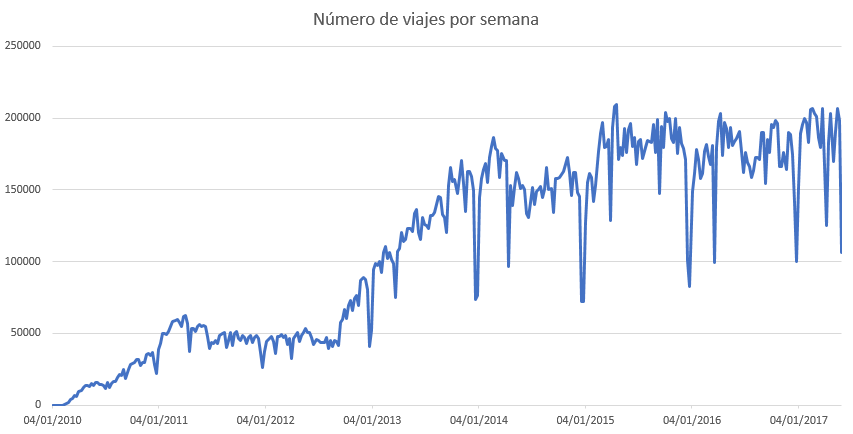
\includegraphics[width=15cm]{Imagenes/viajes_por_semana.png}\\
		\begin{centering}
		\caption{Viajes por semana de Ecobici}
		\end{centering}
	\end{figure}
	Por otro lado, las estaciones parecen tener un comportamiento definido. Durante los últimos 3 años, la estación 27 Reforma Havre ha sido la mayor demandada, superando por mucho al resto de estaciones en número de arribos y salidas.
	\begin{figure}[H]
		\centering
		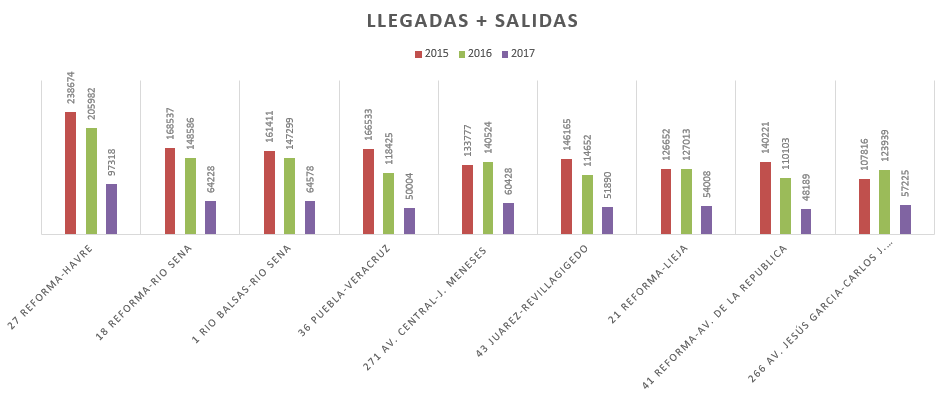
\includegraphics[width=15cm]{Imagenes/estaciones_mayor_actividad.png}\\
		\begin{centering}
		\caption{Estaciones con mayor actividad durante los últimos 3 años}
		\end{centering}
	\end{figure}
	\begin{figure}[H]
		\centering
		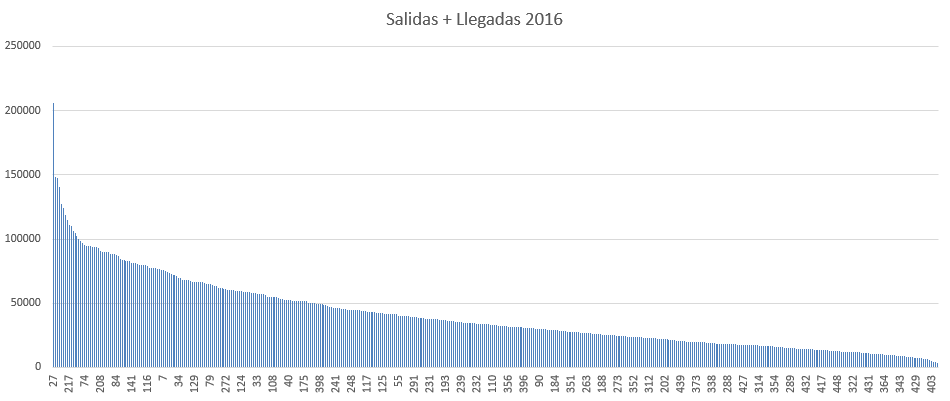
\includegraphics[width=15cm]{Imagenes/salidas_y_llegadas_2016.png}\\
		\begin{centering}
		\caption{Suma de llegadas y salidas en el 2016 por estación}
		\end{centering}
	\end{figure}
	En cambio, si se hace la diferencia entre salidas y llegadas se puede ver que hay estaciones que naturalmente tienen mayor número de salidas que llegadas, otras con más llegadas y un tipo de estación que parece tener un balance entre llegadas y salidas.
	\begin{figure}[H]
		\centering
		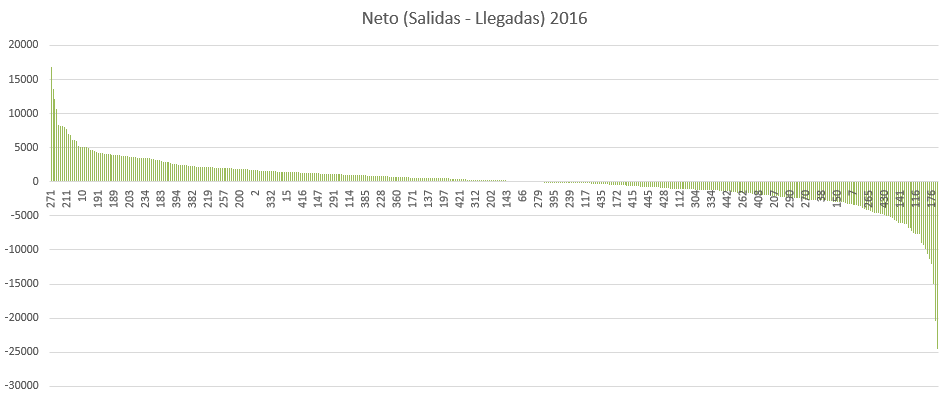
\includegraphics[width=15cm]{Imagenes/salidas_menos_llegadas_2016.png}\\
		\begin{centering}
		\caption{Diferencia entre salidas y llegadas en el 2016 por estación}
		\end{centering}
	\end{figure}
	Aunque esto puede generar una interpretación errónea si no se analiza a mayor profundidad como se hará mas adelante. Por ejemplo las estaciones \textit{266 Av. Jesús García-Carlos J. Meneses} y \textit{267 AV. Jesús García-Carlos J. Meneses} son las que tienen mayor número de llegadas, pero son contiguas a las estaciones \textit{271 AV. Central-J. Meneses} y \textit{272 AV. Central-J. Meneses} las cuales son 1er y 6to lugar en número de salidas respectivamente. Como este hay más casos de estaciones contiguas con flujos recíprocos.\\
	La mayor actividad dentro de la Ciudad de México se genera en avenida Reforma y la zona de Buenavista. Después le siguen las colonias Condesa y Roma Norte.
	\begin{figure}[H]
		\centering
		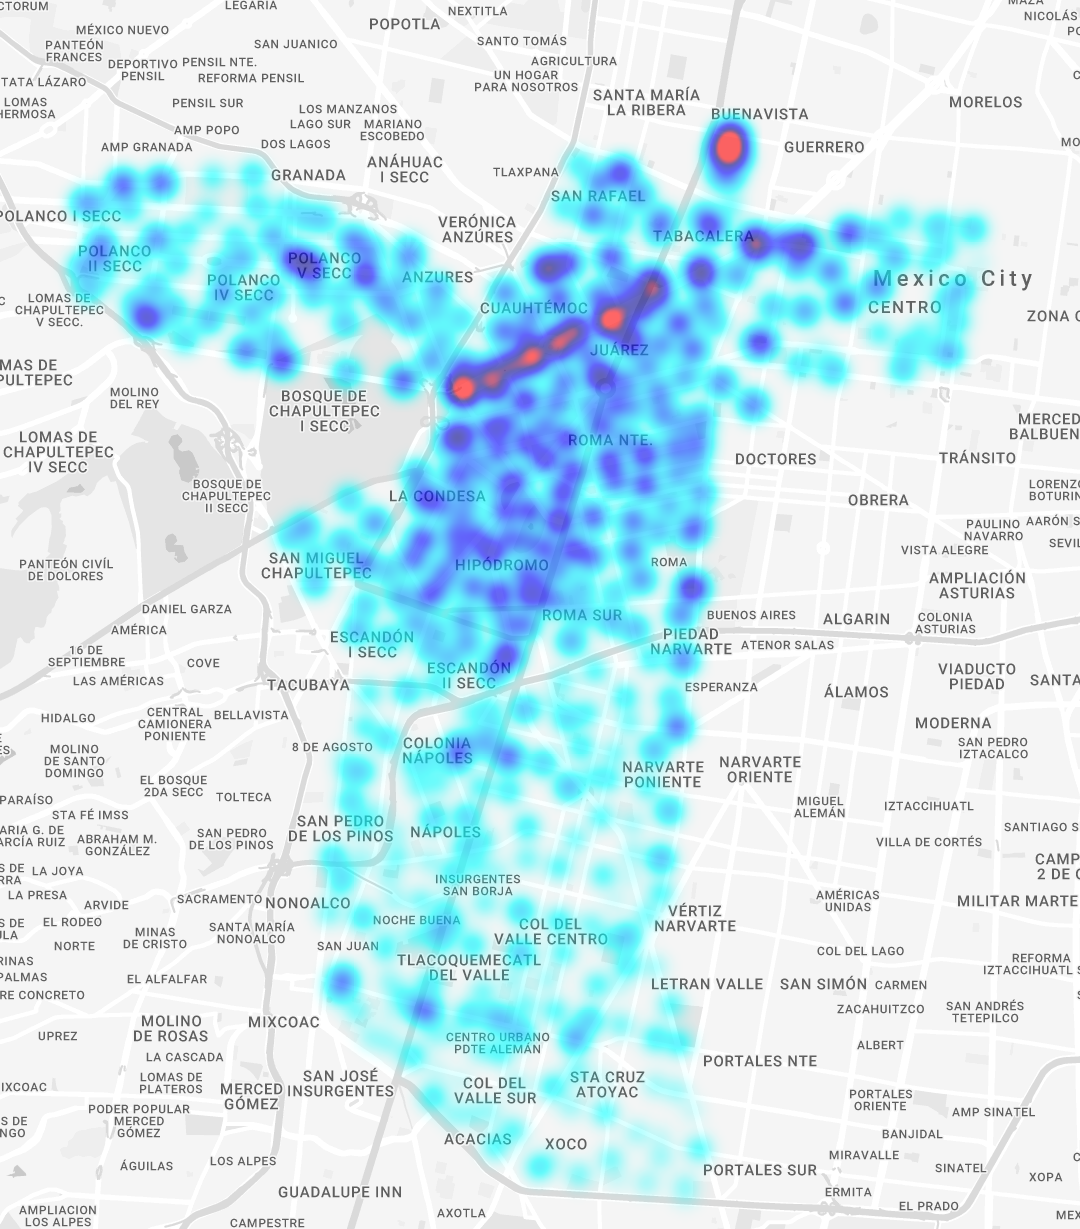
\includegraphics[width=10cm]{Imagenes/HeatmapEcobici2.png}
		\begin{centering}
		\caption{Mapa de calor por llegadas y salidas de los últimos 3 años}
		\end{centering}
	\end{figure}
	Pero los viajes más frecuentes entre 2 estaciones no son en ninguna de las zonas mencionadas. Los más comunes se dan entre la estación \textit{211 Newton-Horacio} y \textit{217 Euler-Av. Horacio} ubicadas en Polanco con poco más de 2300 viajes durante el 2016.\\
	\begin{figure}[H]
		\centering
		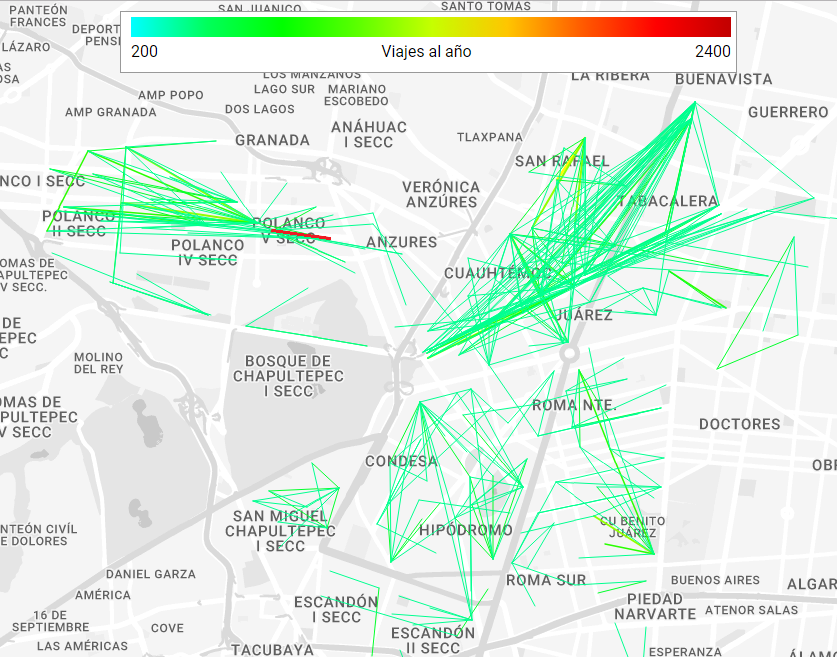
\includegraphics[width=10cm]{Imagenes/viajes_mas_comunes.png}
		\begin{centering}
			\caption{Viajes al año entre 2 estaciones}
		\end{centering}
	\end{figure}
	\begin{table}[H]
		\centering
		\caption{Viajes más comunes durante 2016}
		\label{my-label}
	\begin{tabular}{ | l | l |}
		Estaciones & Total de viajes \\ \hline
		211 - 217 & 2321 \\ \hline
		174-183 & 1631 \\ \hline
		1-18 & 1536 \\ \hline
		85-174 & 1244 \\ \hline
		174-257 & 1216 \\ \hline
		206-208 & 1204 \\ \hline
		21-27 & 1158 \\ \hline
	\end{tabular}
	\end{table}
	\pagebreak
	Parece ser que hay 2 comportamientos en los viajes realizados durante diferentes días de la semana. De Lunes a Viernes el número de viajes totales es parecido, pero disminuye durante los fines de semana. En los últimos 3 años el día martes ha sido el que más viajes ha tenido y domingo el de menor actividad.
	\begin{figure}[H]
		\begin{floatrow}
			\ffigbox{%
				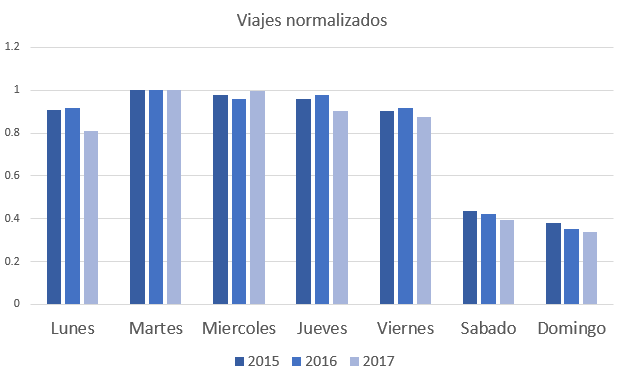
\includegraphics[width=8cm]{Imagenes/viajes_por_dia_semana.png}%
			}{%
				\caption{Viajes por día de la semana}%
			}
			\capbtabbox{%
				\begin{tabular}{ | l | l | l | l |}
					\hline
					& \multicolumn{3}{|c|}{Actividades por año}\\ \cline{2-4}
					& 2015 & 2016 & 2017 \\ \hline
					Lunes & 1500917 & 1501661 & 619677\\ \hline
					Martes & 1651031 & 1636017 & 764333 \\ \hline
					Miercoles & 1613269 & 1572465 & 760441 \\ \hline
					Jueves & 1586421 & 1598553 & 689980 \\ \hline
					Viernes & 1493699 & 1498526 & 667820 \\ \hline
					Sabado & 716738 & 689625 & 300114 \\ \hline
					Domingo & 629794 & 572640 & 258865 \\ \hline
				\end{tabular}
			}{%
			\caption{Viajes por día de la semana}%
			}
		\end{floatrow}
	\end{figure}

	De ahora en adelante se utilizarán solamente 1 conjunto de datos acotado en base a 2 supuestos.
	\begin{enumerate}
		\item Solo se utilizarán los días entre semana ya que son los relevantes para análisis y estudio del sistema.
		\item Se trabajarán solo los años 2015 y 2016 para análisis y estudio ya que la actividad en ambos fue parecida. El año 2017 se utilizará para prueba de hipótesis.
	\end{enumerate}

	\pagebreak
	Todos los días entre semana parecen comportarse de manera parecida; hay un pico de actividad alrededor de las 9:00, disminuye y vuelve a aumentar un poco a las 14:00, finalmente a las 19:00 hay otro pico parecido al de la mañana pero con una disminución gradual. Coincide con el comportamiento de un día laboral: la gente se va a trabajar en la mañana y algunos salen a comer, a las 7 ya es hora de salida. Los días viernes hay menor actividad después de las 5 de la tarde que los otros días.
	\begin{figure}[H]
		\centering
		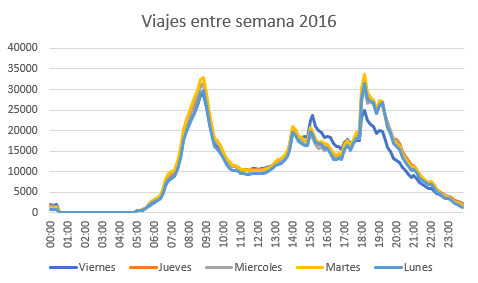
\includegraphics[width=10cm]{Imagenes/viajes_entre_semana_2016.png}
		\begin{centering}
		\caption{Número de viajes en días laborales del 2016}
		\end{centering}
	\end{figure}
	\pagebreak
	Algo que podría complicar aún más el rebalanceo es que los cambios de una semana a otra son mayores a nivel de estación, por ejemplo la estación 27 durante los martes parece tener un flujo controlado (con poca variación) durante las primeras horas del día, pero después de la 1 de la tarde este flujo cambia mucho de un martes a otro. Esto puede deberse a fallos en el rebalanceo, cambios en el clima, comportamiento anormal de la gente o algún otro factor que cambie la demanda de bicicletas para cierta estación.
	\begin{figure}[H]
		\centering
		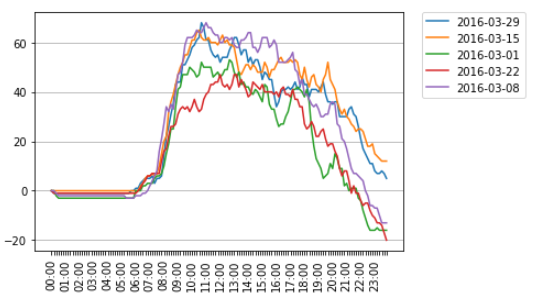
\includegraphics[width=15cm]{Imagenes/27_martes_2.png}
		\begin{centering}
			\caption{Flujo neto (llegadas - salidas) para diferentes martes en la estación 27}
		\end{centering}
	\end{figure}
	\newpage
	\section{Clustering}
	Consiste an agrupar elementos dependiendo de sus similaridades. Tarea que resulta muy útil al separar las estaciones de Ecobici de acuerdo a un criterio. Así resultaría más fácil analizar una sola estación que represente a un grupo en lugar de analizar las 452 estaciones por separado. Hay diversos métodos para separar por clusters, se utilizarán 3 métodos y se compararán resultados.
	\subsection{K Means}
	Algoritmo usado para dividir n observaciones en k grupos de manera que cada grupo tenga una varianza mínima entre sus observaciones. Se puede describir por la siguiente ecuación:\\
	*Ecuacion con errores sintacticos en Latex*
	Se utilizó la librería de Python Scikit para generar clusters de las estaciones dependiendo de su posición geográfica
	\begin{figure}[H]
		\centering
		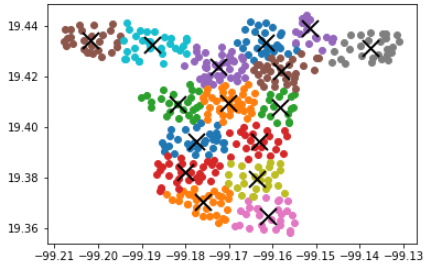
\includegraphics[width=15cm]{Imagenes/kmeans_16.png}
		\begin{centering}
			\caption{K means con 16 clusters}
		\end{centering}
	\end{figure}
	Estos clusters se formaron en base a ubicación geográfica. Qué sucede si añadimos otros factores como salidas y llegadas?
	*Debo hacer algo con los viajes para que se generen mejores clusters*
	\begin{figure}[H]
		\centering
		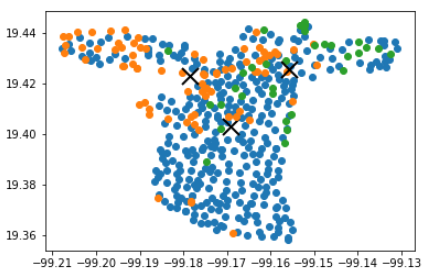
\includegraphics[width=15cm]{Imagenes/kmeans_3.png}
		\begin{centering}
			\caption{K means con 3 clusters usando posicion y llegadas - salidas}
		\end{centering}
	\end{figure}
	\subsection{Affinity Propagation}
	Elige los clusters dependiendo del número de observaciones.
	\begin{figure}[H]
		\centering
		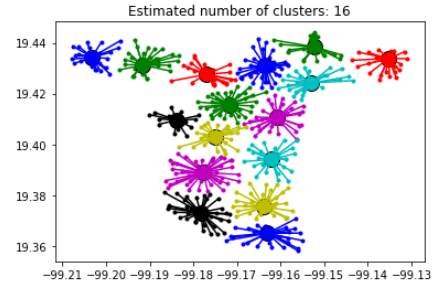
\includegraphics[width=15cm]{Imagenes/ap_16.png}
		\begin{centering}
			\caption{Affinity Propagation genera 16 clusters}
		\end{centering}
	\end{figure}
	\newpage
	\section{Redes neuronales}
	Como se mencionó en la primer sección de este documento, es necesario tener una buena predicción sobre el tráfico en el sistema. Algunos autores han propuesto utilizar redes neuronales para modelar estos problemas [Zhao et. al]. Pero antes es necesario explicar qué es una red neuronal y porqué es factible resolver este tipo de problemas usándolas.\\
	Las redes neuronales son sistemas computacionales diseñados para que por medio de un entrenamiento en base a valores de entrada y sus respectivos valores de salida sean capaces de ``aprender'' una función $ y = y(x) $. Para el entrenamiento se necesita definir \textit{epochs} y tamaño del \textit{batch}.\\
	Un \textit{epoch} es recorrer toda la información de entrenamiento, así a mayor número de epochs se recorre más veces la información de entrenamiento. Un bajo número de epochs puede significar que la red no aprenda la función, por el contrario un número alto puede traer problemas de sobreajuste, siendo incapaz la red de reaccionar a información nueva.\\
	Un \textit{batch} o lote, es una parte de la información de entrenamiento. Entre más grande sea el lote es mayor la memoria computacional necesaria, un número bajo implica mayor número de iteraciones para completar un \textit{epoch}. Por ejemplo si se tienen 1000 ejemplos de entrenamiento y un tamaño de lote de 500 se necesitan 2 iteraciones para completar un \textit{epoch}.\\
	Las redes neuronales están formadas por neuronas artificiales que simulan la conexión dentro un cerebro, donde las neuronas conectadas unas con otras generan enlaces que pueden incrementar o disminuir el estado de activación de las neuronas circundantes. 
	\begin{figure}[H]
		\centering
		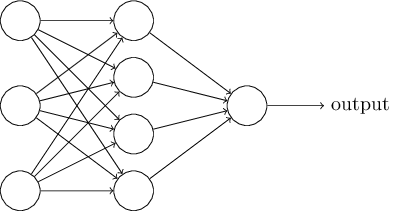
\includegraphics[width=10cm]{Imagenes/neural_network_structure.png}
		\begin{centering}
			\caption{Estructura de una red nueronal simple}
		\end{centering}
	\end{figure}
	
	Como una neurona puede tener múltiples entradas, es necesario que tengan diferente importancia, para esto se multiplica por un valor  \textit{w} (por weight en inglés). Por otro lado cada neurona tiene un umbral de activación \textit{b} (por bias en inglés). Típicamente la función de salida de la neurona es una función sigmoide, esto para poder representar pequeños cambios en las entradas de manera adecuada.
	\[ \sigma(z) = \sigma(wx + b) \tag{1}\]
	Se necesitan encontrar valores para cada \textit{w y b} tal que la salida de la red se aproxime a la función $ y(x)$. Para medir que tan buena es esta aproximación se define una función de costo:
	\[ C(w,b) = \frac{1}{2n}\sum\limits_{x} \norm{y(x) - a}^2 \]
	Donde $ w $ denota todos los \textit{weights} en la red, $ b $ todos los \textit{biases}, $ n $ es el número total de valores de entrada de entrenamiento, $ a $ es la salida de la red para cada entrada $ x $. El $ 1/2 $ se usa por conveniencia para que en la derivada cancele el 2. Cuando $ C(w,b) \approx 0 $ significa que la salida de la red $ a $ es aproximadamente igual a $ y(x) $, por lo que se deben modificar $ w $ y $b$ para minimizar $ C $.\\
	Para encontrar los valores de $w$ y $b$ que minimicen se utiliza un algoritmo llamada \textbf{\textit{gradient descent}}, que funciona calculando el gradiente $ \nabla C$ para mover los valores proporcionalmente en la dirección negativa, así eventualmente se moverán hasta encontrarse en un punto muy cercano al mínimo de la función. Se define con la siguiente ecuación:
	\[ \nabla v = -\eta\nabla C \]
	Donde $v$ representa el vector de variables que definen $C$ y $\eta$ es un valor positivo preferentemente pequeño para que los cambios en $v$ sean graduales, es conocido como \textbf{\textit{learning rate}}. Para realizar los cálculos se utiliza otro algoritmo llamado \textbf{\textit{backpropagation}}.
	\subsection{Algoritmo de Backpropagation}
	El objetivo de este algoritmo es calcular las derivadas parciales $ \partial{C}/\partial{t} $ y $ \partial{C}/\partial{b} $ de la función \textit{C} respecto a cada \textit{w y b} utilizando 4 ecuaciones. Para explicar con más detalle se usará la siguiente nomenclatura:
	\begin{itemize}
		\item $b^l_j$ es el \textit{bias} de la neurona $j$ en la capa $l$.
		\item $w^l_jk$ es el \textit{weight} que va de la neurona $j$ en la capa $l-1$ hacia la neurona $k$ en la capa $l$
		\item $a^l_j$ es la salida o activación de la neurona $j$ en la capa $l$.
	\end{itemize}

	\begin{figure}[H]
		\centering
		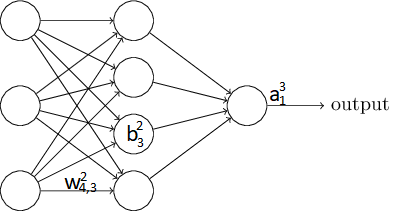
\includegraphics[width=10cm]{Imagenes/neural_network_nomenclature.png}
		\begin{centering}
			\caption{Nomenclatura básica de una red neuronal}
		\end{centering}
	\end{figure}
	Se necesita una ecuación para medir el error en cada capa:
	\[ \delta^L_j = \frac{\partial{C}}{\partial{a^L_j}}\sigma'(z^L_j) \tag{BP1}\]
	Donde $\delta^L_j$ es el error en la neurona $j$ de la capa $L$, $\partial{C}/\partial{a^L_j}$ es el cambio de la función $C$ respecto a la salida de la misma neurona, $\sigma'(z^L_j)$ es el cambio en la función  respecto al vector de entrada $z$ para la neurona $j$ en la capa $L$. Es importante notar que en la ecuación (1) x puede ser sustituida por el vector de activación $a$ de la capa anterior, ya que el objetivo de esta ecuación es obtener el error dado un vector de activación. La ecuación puede reescribirse de forma matricial de la siguiente manera:
	\[ \delta^L = \nabla_a C \odot \sigma'(z^L). \tag{BP1a} \]
	Otra ecuación necesaria es una que permita relacionar los errores entre diferentes capas. Ya que realmente solo se conoce el error de la última capa, es necesario trasladar este error a capas anteriores, para esto se utiliza:
	\[ \delta^l = ((w^{l+1})^T \delta^{l+1}) \odot \sigma'(z^l)	\tag{BP2} \]
	Donde $w^{l+1}$ es la matriz de los \textit{weights} para la capa $l+1$. Si se multiplica $\delta^{l+1}$ -que ya se conoce gracias a la ecuación (BP1)- por la matriz $w$ se está moviendo el error a una capa anterior, $\sigma'(z^l)$ es solo para darle una magnitud a este error.\\
	Combinando la ecuación (BP1) y (BP2) se puede calcular el error para cualquier neurona en la red, ahora solo se necesita relacionar este error con el cambio en $w$ y $b$.
	\[ \frac{\partial C}{\partial b^l_j} =	\delta^l_j.	\tag{BP3} \]
	Esto significa que el error en una neurona es exactamente igual al cambio en el \textit{bias b} de una neurona.\\
	\[ \frac{\partial C}{\partial w^l_{jk}} = a^{l-1}_k \delta^l_j.	\tag{BP4} \]
	La última ecuación establece que el cambio en un \textit{weight w} es igual al vector de activación en la entrada de esta neurona multiplicada por el error.\\
	Usando estas 4 ecuaciones se puede definir el algoritmo para entrenar una red de la siguiente manera:
	\begin{enumerate}
		\item Insertar un grupo de datos de entrenamiento.
		\item Para cada ejemplo de entrenamiento meter los valores a la entrada de la primer capa.
		\item Para cada capa $l=2,3,...,L$ calcular $z^{x,l} = w^l a^{x,l-1}+b^l$ y $\sigma(z)$.
		\item Calcular el error para la última capa con la ecuación (BP1).
		\item Propagar hacia las capas anteriores este error usando (BP2).
		\item Modificar los valores de w y a usando \textbf{\textit{gradient descent}} y las ecuaciones (BP3) y (BP4)
	\end{enumerate}
	\subsection{Recurrent Neural Networks}
	El tipo de redes que se mostró al inicio de esta sección son llamadas \textit{Feedforward Networks} por el modo que funcionan; se insertan datos y en un flujo en una sola dirección estos datos son convertidos en información. No tiene relevancia el orden en que se muestren los datos.\\
	\begin{figure}[H]
		\centering
		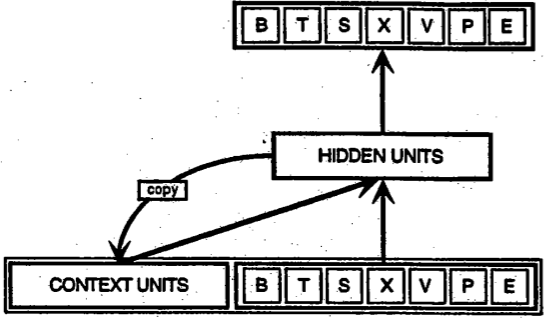
\includegraphics[width=10cm]{Imagenes/rnn_structure.png}
		\begin{centering}
			\caption{Estructura básica de una Red Neuronal Recurrente}
		\end{centering}
	\end{figure}
	En el caso que sea importante la secuencia en la que se insertan los datos existen las llamadas \textit{Recurrent Neural Networks} (RNN). Estas guardan un estado que refleje el flujo histórico de los datos y lo utilizan como retroalimentación. A este estado se le va a llamar \textit{hidden state} y será denotado con $h_t$ donde t es un momento en el tiempo. La ecuación que define a este estado es la siguiente:
	\[ h_t = \phi (Wx_t + Uh_{t-1}) \]
	Donde $h_t$ es el \textit{hidden state} en el tiempo $t$, $\phi$ es una función que puede ser sigmoide o $tanh$, $W$ es la matriz de \textit{weights}, $X_t$ es el vector de entrada en el tiempo t, $U$ es la matriz de transición (lo mismo que \textit{weights} pero para $h$) y $h_{t-1}$ es el vector de hidden states anteriores. \\
	Este tipo de redes utiliza una variación del algoritmo de \textit{Backpropagation} para su entrenamiento conocido como \textit{Backpropagation Through Time} (BPTT), la variación es que debe expandir la función de retroalimentación n veces antes de calcular $y$.
	\begin{figure}[H]
		\centering
		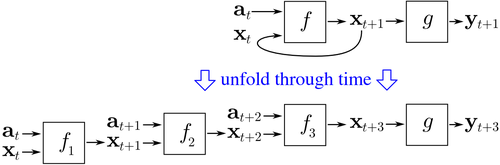
\includegraphics[width=10cm]{Imagenes/bptt.png}
		\begin{centering}
			\caption{Algoritmo de BPTT}
		\end{centering}
	\end{figure}
	El problema que surge con este tipo de redes es que es muy difícil conocer la importancia de un suceso muy remoto porque la información puede pasar por muchas operaciones y se puede ir reduciendo, haciendo muy lento el aprendizaje ya que los cambios son mínimos. Para resolver este problema surgen las llamadas \textbf{\textit{Long Short Term Memory Networks}} (LSTM).
	\begin{figure}[H]
		\centering
		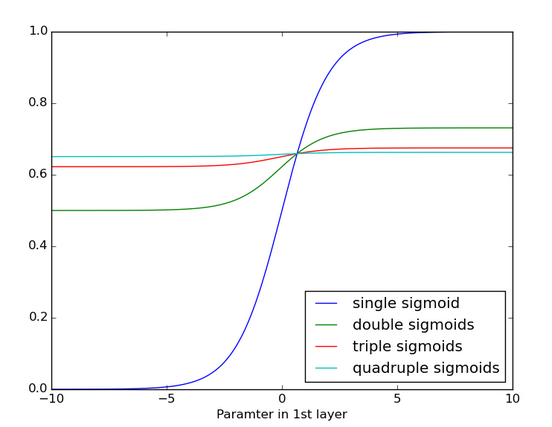
\includegraphics[width=10cm]{Imagenes/sigmoid_vanishing_gradient.png}
		\begin{centering}
			\caption{Efectos de aplicar una función sigmoide múltiples veces}
		\end{centering}
	\end{figure}
	\subsection{LSTM}
	Son un tipo de red que permite el aprendizaje incluso con más de 1000 pasos en el tiempo. Almacenan información dentro una celda, fuera del flujo normal de la red. En esta se puede escribir y leer información por medio de compuertas implementadas con la función sigmoide. Al igual que las neuronas, bloquean o permiten pasar cantidades de información dependiendo de sus propios \textit{weights}, así las celdas aprenden cuándo permitir que la información sea escrita o leída. El siguiente diagrama representa el funcionamiento de una LSTM.\\
	\begin{figure}[H]
		\centering
		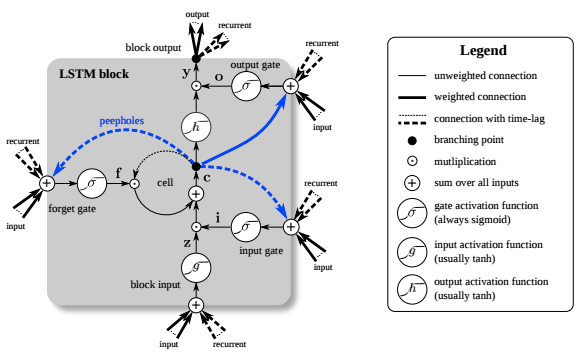
\includegraphics[width=10cm]{Imagenes/lstm_structure.png}
		\begin{centering}
			\caption{Representación de una LSTM}
		\end{centering}
	\end{figure}
	La información del \textit{input} llega por debajo, se le aplica una funcion de aplastamiento como $tanh$. Posteriormente es multiplicada por la información que ya contenía la celda. Se actualiza la información de la celda en cada paso del tiempo, las compuertas pueden decidir que tanto olvidar, escribir o leer de la información.
	\subsection{Implementación de una LSTM para predicción de demanda}
	Una vez que se conocen las bases de una red neuronal, es fácil notar porque estas se pueden utilizar para predicción. La función de demanda a través del tiempo en el BSS de Ecobici resultaría imposible de determinar, pero puede aproximarse con una LSTM.\\
	*Aquí va la descripción de la red*\\
	A continuación se presentan las predicciones de la red para diferente número de \textit{epochs}, en naranja es lo predicho por la red y azul las demandas reales. Cabe recalcar que no hubo una retroalimentación en la predicción para estas gráficas, esto quiere decir que lo predicho por la red no se utilizó para predecir el siguiente paso, en cambio se utilizaron solo los últimos 78 momentos reales.
	\begin{figure}[H]
		\centering
		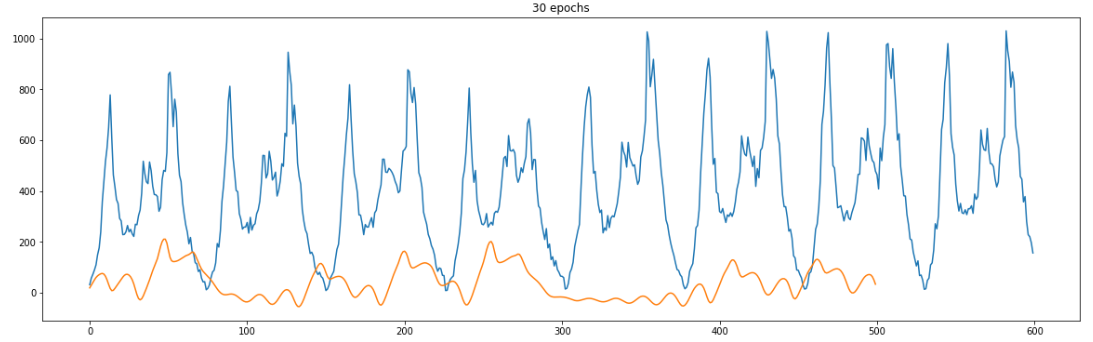
\includegraphics[width=15cm]{Imagenes/full_30_epochs.PNG}
		\begin{centering}
			\caption{Red con 30 epochs de entrenamiento prediciendo demanda para todo el sistema}
		\end{centering}
	\end{figure}
	\begin{figure}[H]
		\centering
		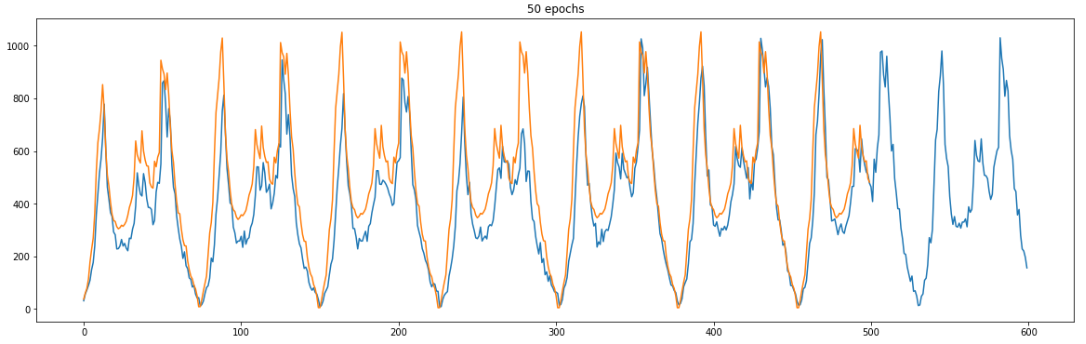
\includegraphics[width=15cm]{Imagenes/full_50_epochs.PNG}
		\begin{centering}
			\caption{Red con 50 epochs de entrenamiento prediciendo demanda para todo el sistema}
		\end{centering}
	\end{figure}
	\begin{figure}[H]
		\centering
		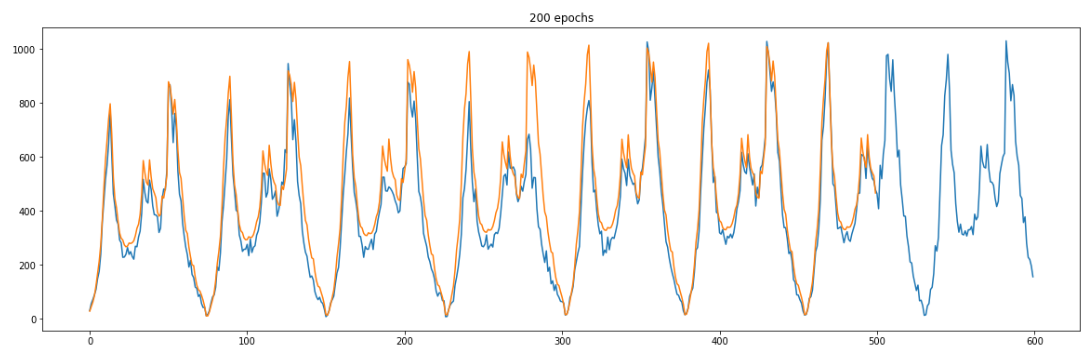
\includegraphics[width=15cm]{Imagenes/full_200_epochs.PNG}
		\begin{centering}
			\caption{Red con 200 epochs de entrenamiento prediciendo demanda para todo el sistema}
		\end{centering}
	\end{figure}
	Si el mismo modelo es utilizado para predecir un día completo con retroalimentación de la red se obtiene el siguiente resultado. Esto significa que cada predicción que va haciendo la red se vuelve a insertar en el vector \textit{input} para predecir el siguiente paso
	\begin{figure}[H]
		\centering
		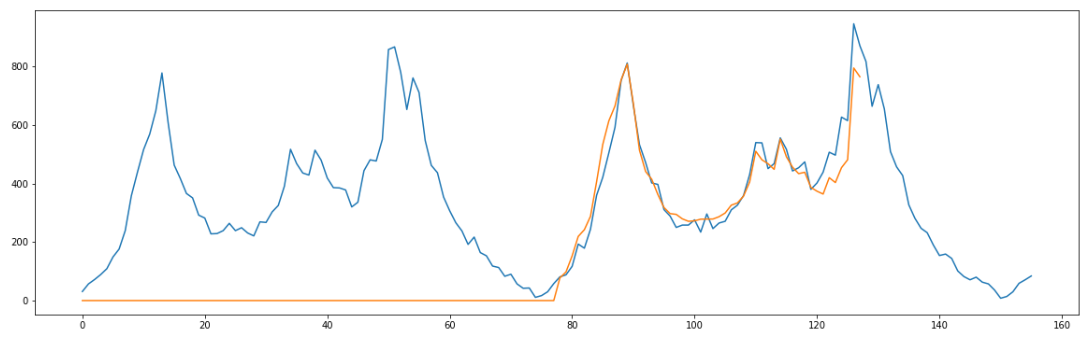
\includegraphics[width=15cm]{Imagenes/model_predict_1_day.PNG}
		\begin{centering}
			\caption{Predicción de casi un día con retroalimentación de la red}
		\end{centering}
	\end{figure}
	Estos son buenos resultados, en cambio si se quiere utilizar el mismo modelo para predecir la demanda en el cluster de Buenavista es notorio que difieren los resultados reales con los predichos.
	\begin{figure}[H]
		\centering
		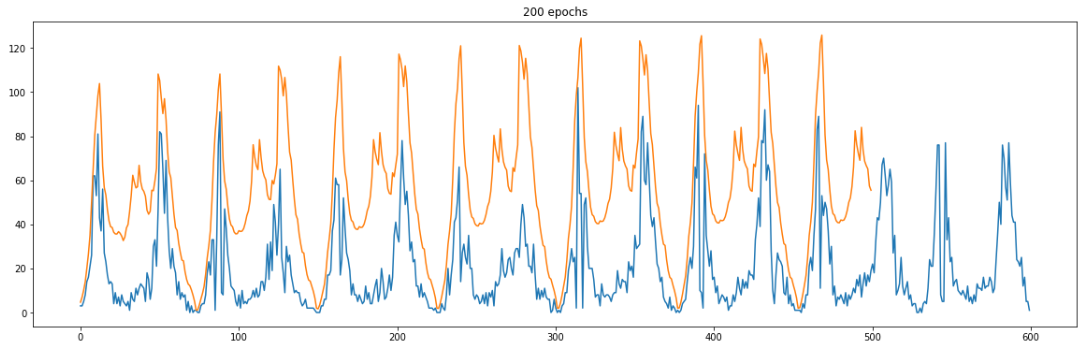
\includegraphics[width=15cm]{Imagenes/model_predict_buenavista_cluster.PNG}
		\begin{centering}
			\caption{Predicción usando el modelo de todo el sistema para predecir solo un cluster}
		\end{centering}
	\end{figure}


	
	\newpage	
	\begin{thebibliography}{9}
		
		\bibitem{lamport94}
		Hazel G. y Miller D. (2007)
		\textit{Desafíos de las Megaciudades},
		\underline{http://www.aan.siemens.com/chile/e-brochures/Documents/Desafío sde las Megaciudades - Siemens.pdf}.
		\bibitem{lamport94}
		Ahmadreza F., Hampshire R., Lavanya M. y Naveen E. (2017) \textit{An empirical analysis of bike sharing usage and rebalancing: Evidence from Barcelona and Seville},Transportation Research Part A, Elsevier.
		\bibitem{lamport94}
		Schuijbroek J., Hampshire R. y Hoeve W. (2013) \textit{Inventory Rebalancing and Vehicle Routing in Bike	Sharing Systems}, Carnegie Mellon University, Estados Unidos.
		\bibitem{lamport94}
		Raviv T. y Kolka O. (2013) \textit{Optimal inventory management of a bike-sharing station}, Taylor \& Francis Ltd.
		\bibitem{lamport94}
		Gebhart K. y Noland R. (2014) \textit{The impact of weather conditions on bikeshare trips in Washington, DC}, Springer Science+Business Media, Nueva York, Estados Unidos.
		\bibitem{lamport94}
		Li Y., Zheng Y., Zhang H. y Chen L. (2014) \textit{Traffic Prediction in a Bike-Sharing System}, Shanghai Jiao Tong University, Shangai, China.
		\bibitem{lamport94}
		Paul DeMaio. \textit(consultado en \textit{The bike sharing world map} Julio de 2017 \underline{https://maps.google.com/maps/ms?ie=UTF8\&hl=en\&om=1\&msa=0\&msid=104227318304000014160.00043d80f9456b3416ced\&ll=43.580391,-42.890625\&spn=143.80149,154.6875\&z=1\&source=embed\&dg=feature}
		\bibitem{lamport94}
		Estadísticas de Ecobici \textit{Traffic Prediction in a Bike-Sharing System}, Shanghai Jiao Tong University, Shangai, China.
		\bibitem{lamport94}
		Zhao Z., Chen W., Wu X., Chen P. y Liu J. \textit{LSTM network: a deep learning approach for short-term traffic forecast}, The Institution of Engineering and Technology.

	
	\end{thebibliography}

\end{document}
%.................................................................................................................................
%=================================================================================================================================
